\documentclass[10pt]{article}
\usepackage{icmlko}

\icmlmeta{IP 파운데이션 월드모델}{229}{섞을 것을 고르는 것이 무게를 고르는 것이다}{무게를 안 고르려고 똑같이 섞는 형태를 쟀다. 무게를 안 고른 것이 아니라 구성원 수로 고르고 있었다}

\begin{document}

\twocolumn[
\icmlheader

\begin{abstract}
노트 228이 과제별 무게를 거절하고 ``무게를 안 고르는 형태부터 재라 ---
셋을 똑같이 1/3 씩, 넷을 1/4 씩''을 남겼다. 열아홉 조합을 다 쟀다.
\textbf{F21$+$F18 이 1 위다}(판 $+$0.4534). \textbf{셋 이상은 전부
아래}이고 넷 이상은 유의하게 아래다(4 형 $-$0.0043 · $t{=}-2.83$, 5 형
$-$0.0068 · $t{=}-2.91$). 왜인지 갈랐더니 \textbf{똑같이 섞는 것이
무게를 안 고르는 것이 아니었다.} 정식화를 선형(F21 · F6 · F9)과 트리
(F18 · F8)로 나누고 조합의 \emph{선형 몫}으로 놓으면 \textbf{노트 227이
쓸어 본 무게 곡선 위에 그대로 놓인다} --- 0.00 $+$0.4399 · 0.33
$+$0.4484 · \textbf{0.50 $+$0.4521} · 0.67 $+$0.4477 · 0.75 $+$0.4427 ·
1.00 $+$0.4360. \textbf{F21$+$F18$+$F6 은 선형 몫 2/3 이고 그것은
$w{=}1/3$ 이다} --- 셋째를 넣는 것은 무게를 옮기는 다른 방법일 뿐이다.
그런데 균형만도 아니다. \textbf{같은 선형 몫 0.50 인데 F21$+$F8 이
$-$0.0052($t{=}-2.60$) · F18$+$F6 이 $-$0.0053($t{=}-2.37$)로 유의하게
진다} --- 계열에서 \emph{제일 좋은 것}이어야 한다. 그리고 균형이 같아도
수를 늘리면 준다(0.50 에서 둘 $+$0.4521 $\to$ 넷 $+$0.4477,
$t{=}-2.83$) --- 약한 구성원이 섞이기 때문이다. \textbf{그러면
``무게를 안 고르는 형태''는 없다.} 있는 것은 하나다 --- \textbf{각
계열에서 제일 좋은 것 하나씩, 둘.} 그것이 이미 F23 이고, 이 노트는 새
형태를 못 찾은 대신 \textbf{F23 이 왜 유일한 무선택 형태인지}를 준다.
\end{abstract}
]

\begin{figure*}[t]
\centering
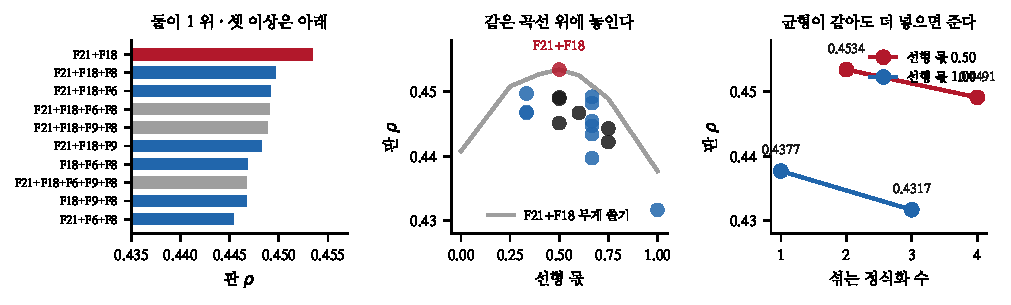
\includegraphics[width=\textwidth]{figs/choosing.pdf}
\caption{왼쪽 --- 둘이 1 위. 가운데 --- 조합이 무게 곡선 위에 놓인다.
오른쪽 --- 균형이 같아도 더 넣으면 준다.}
\end{figure*}

\section{셋 이상은 전부 아래다}

\begin{table}[t]
\centering\tsize
\caption{열아홉 조합(윗부분). 짝 붓스트랩 500 회, F23 대비.}
\begin{tabular}{lrrrr}
\toprule
& 판 & 선형 몫 & 차 & $t$ \\
\midrule
\textbf{F21$+$F18} & \textbf{.4534} & 0.50 & --- & --- \\
F21$+$F18$+$F8 & .4497 & 0.33 & $-$.0036 & $-$1.39 \\
F21$+$F18$+$F6 & .4492 & 0.67 & $-$.0043 & $-$1.80 \\
F21$+$F18$+$F6$+$F8 & .4491 & 0.50 & $-$.0043 & \textbf{$-$2.83} \\
F21$+$F18$+$F9$+$F8 & .4489 & 0.50 & $-$.0045 & \textbf{$-$2.88} \\
\textbf{F21$+$F8} & .4468 & \textbf{0.50} & $-$.0052 & \textbf{$-$2.60} \\
\textbf{F18$+$F6} & .4468 & \textbf{0.50} & $-$.0053 & \textbf{$-$2.37} \\
다섯 전부 & .4467 & 0.60 & $-$.0068 & \textbf{$-$2.91} \\
\bottomrule
\end{tabular}
\end{table}

\claimx{\textbf{F21$+$F18 이 열아홉 조합 전부를 이긴다.} 넷 이상은
유의하게 아래고, 셋은 아래이되 $t$ 가 $-$1.4$\sim$$-$1.8 이다.}{노트
228이 ``무게를 안 고르는 형태''를 기대했는데 \textbf{그 형태들이 다 지금
것보다 못하다.}}

\section{똑같이 섞는 것이 무게를 고르는 것이다}

\begin{table}[t]
\centering\tsize
\caption{선형 몫별 최고 판. 노트 227의 무게 쓸기와 같은 곡선.}
\begin{tabular}{lrl}
\toprule
선형 몫 & 최고 판 & 조합 \\
\midrule
0.00 & .4399 & F18 \\
0.33 & .4484 & F21$+$F18$+$F8 \\
\textbf{0.50} & \textbf{.4521} & \textbf{F21$+$F18} \\
0.60 & .4453 & 다섯 전부 \\
0.67 & .4477 & F21$+$F18$+$F6 \\
0.75 & .4427 & F21$+$F18$+$F6$+$F9 \\
1.00 & .4360 & F21 \\
\bottomrule
\end{tabular}
\end{table}

\claimx{\textbf{조합의 선형 몫으로 놓으면 노트 227의 무게 곡선 위에
놓인다} --- 0.50 에서 최고이고 양쪽으로 내려간다. \textbf{F21$+$F18$+$F6
은 선형 몫 2/3 이고 그것은 $w{=}1/3$ 이다.}}{\textbf{셋째를 넣는 것은
무게를 옮기는 다른 방법일 뿐이다.} 노트 228이 ``대칭 기본값은 고른 것이
아니므로 규약을 안 건드린다''고 적었는데, \emph{무엇을} 대칭으로 놓느냐가
이미 선택이었다.}

\section{균형만도 아니다}

\claimx{\textbf{같은 선형 몫 0.50 인데 F21$+$F8 이 $-$0.0052($t{=}-2.60$)
· F18$+$F6 이 $-$0.0053($t{=}-2.37$)로 유의하게 진다.} 계열에서
\emph{제일 좋은 것}이어야 한다.}{F8 은 F18 보다 판이 $-$0.0103 낮고
F6 는 F21 보다 $-$0.0127 낮다 --- \textbf{약한 대표를 세우면 그 계열이
기여하는 것도 약해진다.}}

\claimx{\textbf{그리고 균형이 같아도 수를 늘리면 준다} --- 선형 몫
0.50 에서 둘 $+$0.4521 $\to$ 넷 $+$0.4477($t{=}-2.83$), 선형 몫 1.00
에서 하나 $+$0.4360 $\to$ 셋 $+$0.4317.}{\textbf{두 손해가 겹친다} ---
셋째를 넣으면 무게가 밀리고 약한 것이 섞인다. 어느 쪽도 안 고르려면
\textbf{계열마다 최고 하나씩}이어야 한다.}

\section{무선택 형태는 하나뿐이다}

\claimx{\textbf{``무게를 안 고르는 형태''는 없다.} 있는 것은 하나다 ---
각 계열에서 제일 좋은 것 하나씩, 둘. \textbf{그것이 이미 F23 이다.}}
{이 노트는 새 형태를 못 찾았고, 대신 \textbf{F23 이 왜 유일한 무선택
형태인지}를 준다 --- 계열이 둘이고 각 계열의 대표가 정해지면 남는
자유도가 없다.}

\claimx{\textbf{계열이 둘이라는 것도 잰 것이다}(노트 225) --- 다섯
정식화가 두 과제에서 완전히 역순이었고 그 경계가 선형 대 트리였다.}
{\textbf{그래서 이 형태는 노트 225$\to$226$\to$227$\to$229 가 한 줄로
이어진 것이다} --- 계열이 둘임을 보고, 왜 갈리는지 알고(풀링 이득),
섞고, 섞을 것이 왜 둘뿐인지 확인했다.}

\begin{table}[t]
\centering\tsize
\caption{남은 것.}
\begin{tabular}{ll}
\toprule
\textbf{셋째 계열} & 선형·트리 말고 다른 계열을 세울 수 있나 \\
\textbf{F21 개선} & 계열 대표가 좋아지면 F23 도 좋아진다 \\
웹툰 & F23 도 웹툰이 $+$0.3828 로 제일 낮다 \\
\bottomrule
\end{tabular}
\end{table}

첫 줄이 이 노트가 남기는 유일한 열린 길이다. \textbf{F23 의 천장은 두
계열의 대표가 정한다} --- 선형과 트리 말고 \emph{셋째 계열}이 있으면 판이
0.50/0.50 에서 1/3 씩으로 넓어진다. 후보는 포트폴리오에 이미 있다 ---
F2 결합 잠재(도메인을 잠재 공간으로 묶는다)와 F9 순위 우도(제곱오차가
아니라 짝 순위로 맞춘다)다. \textbf{F9 는 이 노트에서 선형으로 묶었는데
목적함수가 다르므로 따로 세워 볼 값이 있다} --- 다만 F9 를 넣은 조합이
전부 아래였으므로(F21$+$F18$+$F9 $-$0.0053) \textbf{계열이 다르다는 것과
기여가 다르다는 것은 다른 말이고, 그것부터 재야 한다.}

\end{document}
